\providecommand{\Fun}{\operatorname{Fun}}
\providecommand{\QCat}{\mathcal{Q}\mathcal{C}at}
\providecommand{\CSS}{\mathcal{CSS}}
\providecommand{\Cat}{\mathcal{C}at}
\providecommand{\rvTfibArrow}{\mathrel{\stackrel{\sim}{\twoheadrightarrow}}}
\providecommand{\rvEqArrow}{\mathrel{\stackrel{\sim}{\Rightarrow}}} %
\section{\trCosmologicalFunctor}\label{sec:cosmological-functors}

某些「右\trAdjunction{}型」的构造定义了\trInfinityCosmos{}之间的映射，
这些映射保持定义 1.2.1 中公理化的全部结构。%
这类构造定义\trInfinityCosmos{}之间的\emph{\trCosmologicalFunctor}
（cosmological functor）——这一简单的观察使许多证明变得精简。

\begin{definition}[\trCosmologicalFunctor]\label{def:cosmological-functor}
\textbf{\trCosmologicalFunctor}是一个\trInfinityCosmos{}之间的
\textbf{\trSimplicialFunctor}（simplicial functor；见定义 A.2.6），%
它保持指定的\trIsofibration{}与全部宇宙论\trLimit{}。
\end{definition}

一般地，\trCosmologicalFunctor{}保持任何能在\trInfinityCosmos{}\emph{内部}刻画的
∞-范畴论概念——例如，作为配有附加结构的映射——与之相对的是
\emph{外部}刻画的概念——例如，由一条涉及全称量词或存在量词的
陈述所作的刻画。例如，\trInfinityCosmos{}中的\trEquivalence{}%
在定义 1.2.2 中是外部刻画的，%
这可能让人怀疑，一个非满射的\trCosmologicalFunctor{}或许无法保持它们。
然而，引理 1.2.15 把\trEquivalence{}刻画为\trInfinityCosmos{}内部
定义的诸结构之存在性，%
于是作为结论：

\begin{lemma}\label{lem:cosmological-preserves-equivalences}
任何\trCosmologicalFunctor{}还保持\trEquivalence{}与\trTrivialFibration{}。
\end{lemma}
\begin{proof}
由引理 1.2.15，%
\trInfinityCosmos{}中的\trEquivalence{}与「\trHomotopy\trEquivalence」重合，
后者由与\trFreeLivingIsomorphism{}作\trCotensor{}来定义。由于\trCosmologicalFunctor{}保持单纯\trCotensor{}，
它保持 (1.2.16) 中所示的数据，%
从而把\trEquivalence{}送到\trEquivalence{}。\trTrivialFibration{}的保持随之而得。
\end{proof}

\begin{remark}\label{rem:cosmological-discrete-categories}
类似地，单从定义 1.2.26 出发论证，%
并不清楚\trCosmologicalFunctor{}是否保持离散\trInfinityCategory{}；
但利用引理 1.2.27 的内部刻画——%
\trInfinityCategory{} $A$ 是\trDiscrete{}，当且仅当
$A^{\mathbb{I}}\rvTfibArrow A^{\mathbf{2}}$ 是\trTrivialFibration——
这一点便由\trCosmologicalFunctor{}保持单纯\trCotensor{}与\trTrivialFibration{}的事实得出。
\end{remark}

我们现在证明\trCosmologicalFunctor{}是大量存在的：

\begin{proposition}\label{prop:cosmological-functor-constructions}
下列构造对任何\trInfinityCosmos{} $\mathcal{K}$ 都定义\trCosmologicalFunctor{}：
\begin{enumerate}[label=(\roman*)]
\item \trFunctorSpace $\Fun(X,-)\colon\mathcal{K}\to\QCat$，
  对任何\trInfinityCategory{} $X$。
\item \textbf{底\trQuasiCategory}（underlying quasi-category）\trFunctor
  \[
  (-)_0\coloneqq\Fun(1,-)\colon\mathcal{K}\to\QCat,
  \]
  即把 (i) 特化到\trTerminal{}\trInfinityCategory{} $1$。
\item 单纯\trCotensor $(-)^U\colon\mathcal{K}\to\mathcal{K}$，
  对任何\trSimplicialSet $U$。
\item 指数 $(-)^A\colon\mathcal{K}\to\mathcal{K}$，对\trCartesianClosed
  \trInfinityCosmos{} $\mathcal{K}$ 中任何\trInfinityCategory{} $A$。
\item 沿\trInfinityCosmos{} $\mathcal{K}$ 中任何\trFunctor{}
  $f\colon A\to B$ 取\trIsofibration{}的\trPullback
  $f^\ast\colon\mathcal{K}_{/B}\to\mathcal{K}_{/A}$。
\item 而且，对任何\trCosmologicalFunctor $F\colon\mathcal{K}\to\mathcal{L}$
  与任何\trInfinityCategory{} $A\in\mathcal{K}$，
  切片上诱导的映射 $F\colon\mathcal{K}_{/A}\to\mathcal{L}_{/FA}$
  定义一个\trCosmologicalFunctor{}。
\end{enumerate}
\end{proposition}

\begin{proof}
这前四条陈述几乎是立即可得的：\trIsofibration{}的保持在其中每个情形
都被显式断言为一条假设，而\trLimit{}的保持则来自熟悉的论证。

对 (v)，\trInfinityCosmos{} $\mathcal{K}$ 中的\trPullback{}是一个单纯富集的%
\trLimit{}构造；它的一个后果是%
$f^\ast\colon\mathcal{K}_{/B}\to\mathcal{K}_{/A}$
定义一个\trSimplicialFunctor{}。\trFunctor{} $f^\ast$ 在 $\mathcal{K}_{/B}$ 中
0-箭头 $g$ 上的作用同样由一个\trPullback{}方块定义：由于所示图表的前、后
两个方块都是\trPullback{}，顶上的方块亦然
\begin{equation*}
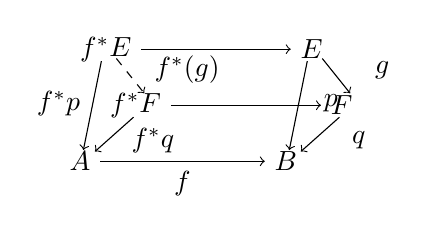
\begin{tikzpicture}[x=1.55em,y=1.35em]
  \node (fsE) at (0.6,3)   {$f^\ast E$};
  \node (E)   at (5.4,3)   {$E$};
  \node (fsF) at (1.3,1.5) {$f^\ast F$};
  \node (F)   at (6.1,1.5) {$F$};
  \node (A)   at (0,0)     {$A$};
  \node (B)   at (4.8,0)   {$B$};
  \draw[->] (fsE) -- (E);
  \draw[->] (fsF) -- (F);
  \draw[->] (A) -- (B) node[midway,below]{$f$};
  \draw[->] (0.5,2.68) -- (0.08,0.3);
  \node at (-0.5,1.55) {$f^\ast p$};
  \draw[->,dashed] (0.85,2.75) -- (1.5,1.82);
  \node at (2.5,2.45) {$f^{\ast}(g)$};
  \draw[->] (1.25,1.18) -- (0.35,0.26);
  \node at (1.7,0.55) {$f^\ast q$};
  \draw[->] (5.3,2.68) -- (4.88,0.3);
  \node at (5.85,1.55) {$p$};
  \draw[->] (5.65,2.75) -- (6.3,1.82);
  \node at (7.05,2.45) {$g$};
  \draw[->] (6.05,1.18) -- (5.15,0.26);
  \node at (6.5,0.55) {$q$};
  \node at (1.05,2.6) {$\scriptstyle\lrcorner$};
  \node at (1.75,1.32) {$\scriptstyle\lrcorner$};
\end{tikzpicture}
\end{equation*}
由于\trIsofibration{}在\trPullback{}下稳定，可知
$f^\ast\colon\mathcal{K}_{/B}\to\mathcal{K}_{/A}$
保持\trIsofibration{}。剩下要证这个\trFunctor{}保持
命题 1.2.22 中构造的那些单纯\trLimit{}，%
而这根本上是\trLimit{}构造之交换性的一个后果。
每种情形都可以显式验证。我们以构造交换立方体为例，
演示单纯\trCotensor{}情形的这一计算：
\begin{equation*}
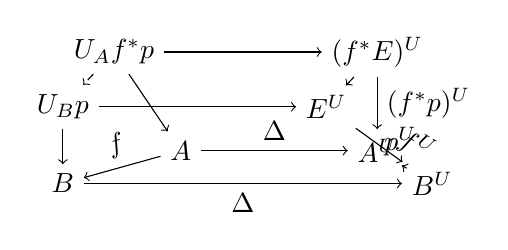
\begin{tikzpicture}[x=1.42em,y=1.32em]
  \node (tfl) at (1.3,3.6) {$U\pitchfork_A f^\ast p$};
  \node (tfr) at (8.0,3.6) {$(f^\ast E)^U$};
  \node (tbl) at (0,2.1)   {$U\pitchfork_B p$};
  \node (tbr) at (6.7,2.1) {$E^U$};
  \node (bfl) at (3.0,0.9) {$A$};
  \node (bfr) at (8.0,0.9) {$A^U$};
  \node (bbl) at (0,0)     {$B$};
  \node (bbr) at (9.4,0)   {$B^U$};
  \draw[->] (tfl) -- (tfr);
  \draw[->,dashed] (tfl) -- (tbl);
  \draw[->] (tbl) -- (tbr);
  \draw[->] (tfr) -- (tbr);
  \draw[->] (tfl) -- (bfl);
  \draw[->] (tbl) -- (bbl);
  \draw[->] (tfr) -- (bfr) node[midway,right]{$(f^\ast p)^U$};
  \draw[->] (tbr) -- (bbr) node[pos=0.4,right]{$p^U$};
  \draw[->] (bfl) -- (bfr) node[midway,above]{$\Delta$};
  \draw[->] (bbl) -- (bbr) node[midway,below]{$\Delta$};
  \draw[->] (bfl) -- (bbl) node[pos=0.5,above,sloped]{$f$};
  \draw[->] (bfr) -- (bbr) node[pos=0.5,above,sloped]{$f^U$};
  \node at (2.5,3.32) {$\scriptstyle\lrcorner$};
  \node at (0.42,1.82) {$\scriptstyle\lrcorner$};
  \node at (7.7,3.3) {$\scriptstyle\lrcorner$};
\end{tikzpicture}
\end{equation*}
由于前、后、右三个面都是\trPullback{}，左面亦然。
最后一条陈述 (vi) 留作\cref{ex:slice-induced-cosmological}。
\end{proof}

\begin{example}\label{exa:cat-kan-cosmological-embeddings}
由命题 1.2.11 与 1.2.12，%
满子\trCategory{}包含 $\Cat\hookrightarrow\QCat$ 与
$\mathcal{K}an\hookrightarrow\QCat$ 都定义\trCosmologicalFunctor
（另见引理 6.1.4）。%
这些\trCosmologicalEmbedding{}阐明了如下直觉：1-\trCategory{}或\trInfinityGroupoid{}的形式范畴论
可以作为 $(\infty,1)$-\trCategory{}的形式范畴论之特例而恢复。
\end{example}

\trCosmologicalFunctor{}的非例同样富有教益： %

\begin{nonexample}\label{exa:forgetful-not-cosmological}
遗忘\trFunctor{} $\mathcal{K}_{/B}\to\mathcal{K}$ 是单纯的
且保持\trIsofibration{}，却并\emph{不}定义\trCosmologicalFunctor{}：
它不保持\trCotensor{}与积。然而，
由\cref{prop:cosmological-functor-constructions}(v)，
其右\trAdjunction{} $-\times B\colon\mathcal{K}\to\mathcal{K}_{/B}$
确实定义一个\trCosmologicalFunctor{}。
\end{nonexample}

\begin{nonexample}\label{exa:core-not-cosmological}
\trCosmologicalEmbedding $\mathcal{K}an\hookrightarrow\QCat$ 有一个右\trAdjunction{}
$(-)^{\simeq}\colon\QCat\to\mathcal{K}an$，它把每个\trQuasiCategory{}%
送到其「\trInfinityGroupoidCore」——即\trMaximalSubKanComplex{}，%
由那些所有边皆为\trIsomorphism{}的 $n$-单纯形组成的单纯子集。
这一核\trFunctor{}保持\trIsofibration{}与 1-范畴论的\trLimit{}，
却不是\trCosmologicalFunctor{}，因为它不是单纯富集的：
任何定义域为\trKanComplex{}而陪域为\trQuasiCategory{}的\trFunctor{}
$K\to Q$ 都经由一个唯一的映射 $K\to Q^{\simeq}$
分解而穿过包含 $Q^{\simeq}\hookrightarrow Q$，
但一般地 $\Fun(K,Q)\ncong\Fun(K,Q^{\simeq})$，
因为\trNaturalTransformation $K\times\Delta[1]\to Q$
只有在其各分量都可逆时才穿过 $Q^{\simeq}\hookrightarrow Q$ 分解
（不过见引理 12.1.12）。%
\end{nonexample}

某些\trCosmologicalFunctor{}的表现格外良好：

\begin{definition}[宇宙论\trBiequivalence{}]\label{def:cosmological-biequivalence}
一个\trCosmologicalFunctor{}定义一个\textbf{宇宙论\trBiequivalence}
（cosmological biequivalence）
$F\colon\mathcal{K}\Rightarrow\mathcal{L}$，如果它还
\begin{enumerate}[label=(\roman*)]
\item 是\textbf{对象在\trEquivalence{}意义下本质满射的}
  （essentially surjective on objects up to equivalence）：
  对一切 $C\in\mathcal{L}$，存在 $A\in\mathcal{K}$
  使得 $FA\simeq C$，并且
\item 定义一个\textbf{局部\trEquivalence}（local equivalence）：
  对一切 $A,B\in\mathcal{K}$，$F$ 在\trFunctorSpace{}上的作用定义%
  \trQuasiCategory{}的\trEquivalence
  \[
  \Fun(A,B)\xrightarrow{\ \sim\ }\Fun(FA,FB).
  \]
\end{enumerate}
\end{definition}

宇宙论\trBiequivalence{}在第 10 章中得到更系统的研究，
在那里我们把它们设想为「\trChangeOfModel{}」\trFunctor{}。
对我们在第 11 章中证明 $(\infty,1)$-范畴论的
「\trModelIndependence{}」而言至关重要的是，
在 $(\infty,1)$-\trCategory{}的诸\trInfinityCosmos{}之间
存在着多种多样的宇宙论\trBiequivalence{}：

\begin{example}[附录 E.2]\label{exa:biequivalences-models}
\begin{enumerate}[label=(\roman*)]
\item 定义在\trCompleteSegalSpaces{}、\trSegalCategories{}与\trOneComplicialSets{}的
  诸\trInfinityCosmos{}上的底\trQuasiCategory\trFunctor
  \[
  \CSS\xrightarrow{\;(-)_0\;}\QCat\qquad
  \mathcal{S}egal\xrightarrow{\;(-)_0\;}\QCat\qquad
  1\text{-}\mathcal{C}omp\xrightarrow{\;(-)_0\;}\QCat
  \]
  都是\trBiequivalence{}。前两种情形由「在第 0 行取值」定义，
  最后一种情形则由「遗忘标记」定义。
\item 还有由 Joyal 与 Tierney \cite{bib64} 定义的宇宙论\trBiequivalence{}
  $\mathrm{nerve}\colon\QCat\Rightarrow\CSS$
  与 $\mathrm{nerve}\colon\QCat\Rightarrow\mathcal{S}egal$。
\item 由 Bergner \cite{bib14} 定义、把\trCompleteSegalSpaces
  「离散化」的\trFunctor{}
  $\mathrm{disc}\colon\CSS\Rightarrow\mathcal{S}egal$
  也定义一个宇宙论\trBiequivalence{}。
\item 另一个宇宙论\trBiequivalence{}
  $(-)^{\flat}\colon\QCat\Rightarrow 1\text{-}\mathcal{C}omp$
  给每个\trQuasiCategory{}配上其「自然标记」。
\end{enumerate}
\end{example}

用命题 10.2.1 所证成的术语来说： %

\begin{definition}\label{def:cosmos-of-infinity-one-categories}
一个\trInfinityCosmos{} $\mathcal{K}$ 是
\textbf{$(\infty,1)$-\trCategory{}的\trInfinityCosmos}
（$\infty$-cosmos of ($\infty$,1)-categories），
当且仅当底\trQuasiCategory\trFunctor $(-)_0\colon\mathcal{K}\to\QCat$
是一个宇宙论\trBiequivalence{}。
\end{definition}

\begin{remark}\label{rem:underlying-qcat-internal-homs}
底\trQuasiCategory\trFunctor $(-)_0\colon\mathcal{K}\to\QCat$
把笛卡尔封闭\trInfinityCosmos{} $\mathcal{K}$ 的\trInternalHom
送到相应的\trFunctorSpace{}：对 $\mathcal{K}$ 中任何\trInfinityCategory{}
$A$ 与 $B$，我们有
\[
(B^A)_0\coloneqq\Fun(1,B^A)\cong\Fun(A,B).
\]
\end{remark}
在\trInfinityCosmos{} $\mathcal{K}$ 与 $\QCat$
\trBiequivalence{}的情形，
我们在第 10 章与第 11 章中将会看到，
这不造成范畴论信息的本质损失。

宇宙论\trBiequivalence{}不仅保持\trEquivalence{}，还会反映并创造它们。

\begin{lemma}\label{lem:biequivalence-reflect-create}
设 $F\colon\mathcal{K}\Rightarrow\mathcal{L}$
是一个宇宙论\trBiequivalence{}。那么：
\begin{enumerate}[label=(\roman*)]
\item $\mathcal{K}$ 中\trInfinityCategory{}之间的\trFunctor{}
  $f\colon A\to B$ 是\trEquivalence{}，当且仅当
  $Ff\colon FA\rvEqArrow FB$ 是 $\mathcal{L}$ 中的\trEquivalence{}。
\item $\mathcal{K}$ 中的一对\trInfinityCategory{}是\trEquivalence{}的，
  当且仅当它们在 $\mathcal{L}$ 中的像是\trEquivalence{}的。
\end{enumerate}
\end{lemma}
\begin{proof}
\cref{lem:cosmological-preserves-equivalences} 蕴含：
\trCosmologicalFunctor{}保持\trEquivalence{}，因而也保持 $\mathcal{K}$ 中
一对\trInfinityCategory{}之间\trEquivalence{}的存在性。
为见\trEquivalence{}也被反映，设 $f\colon A\to B$
是 $\mathcal{K}$ 中一个\trFunctor{}，具有如下性质：
$Ff\colon FA\rvEqArrow FB$ 是 $\mathcal{L}$ 中的\trEquivalence{}。
现在对任何\trInfinityCategory{} $X$，
\trSimplicialFunctor{}性给出交换方块
\begin{equation*}
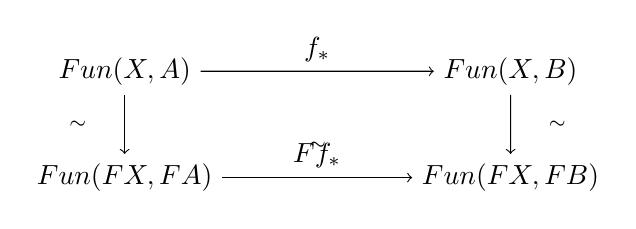
\begin{tikzpicture}[xscale=1.75,yscale=1.35]
\node (TL) at (0,1) {$\Fun(X,A)$};
\node (TR) at (2.8,1) {$\Fun(X,B)$};
\node (BL) at (0,0) {$\Fun(FX,FA)$};
\node (BR) at (2.8,0) {$\Fun(FX,FB)$};
\draw[->] (TL) -- (TR) node[midway,above]{$f_\ast$};
\draw[->] (TL) -- (BL);
\node at (-0.34,0.5) {$\scriptstyle\sim$};
\draw[->] (TR) -- (BR);
\node at (3.14,0.5) {$\scriptstyle\sim$};
\draw[->] (BL) -- (BR) node[midway,above]{$Ff_\ast$};
\node at (1.4,0.3) {$\scriptstyle\sim$};
\end{tikzpicture}
\end{equation*}

于是由\trTwoOfThreeProperty{}可得
$f_\ast\colon\Fun(X,A)\rvEqArrow\Fun(X,B)$ 是\trEquivalence{}，
这就证明了 $f$ 是 $\mathcal{K}$ 中的\trEquivalence{}。

为见\trEquivalence{}也会被创造，现在设 $A$ 与 $B$
是 $\mathcal{K}$ 中配有\trEquivalence{}的\trInfinityCategory
\begin{equation*}
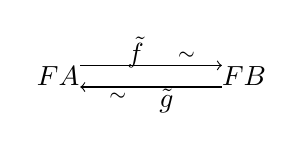
\begin{tikzpicture}[x=1.6em,y=1.3em]
  \node (FA) at (0,0) {$FA$};
  \node (FB) at (4.2,0) {$FB$};
  \draw[->] (0.5,0.3) -- (3.7,0.3);
  \node at (1.75,0.66) {$\tilde{f}$};
  \node at (2.9,0.56) {$\scriptstyle\sim$};
  \draw[->] (3.7,-0.3) -- (0.5,-0.3);
  \node at (2.45,-0.68) {$\tilde{g}$};
  \node at (1.35,-0.58) {$\scriptstyle\sim$};
\end{tikzpicture}
\end{equation*}
\begin{equation*}
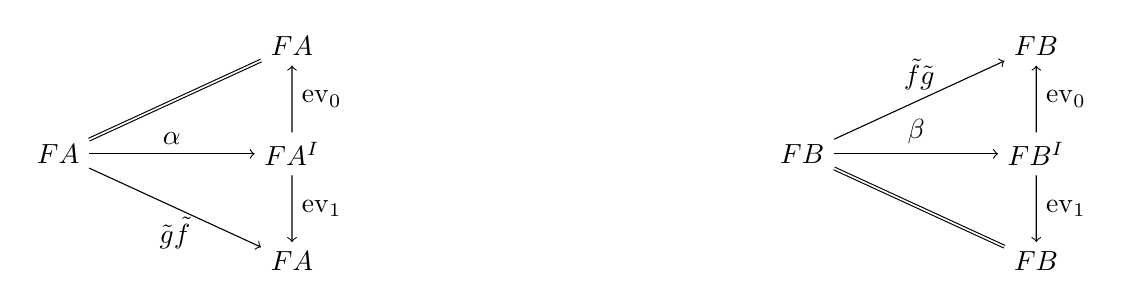
\begin{tikzpicture}[xscale=1.35,yscale=1.05]
\node (lA) at (0,0) {$FA$};
\node (tA) at (2.2,1.3) {$FA$};
\node (Ai) at (2.2,0) {$FA^{\mathbb{I}}$};
\node (bA) at (2.2,-1.3) {$FA$};
\draw[double] (lA) -- (tA);
\draw[->] (Ai) -- (tA) node[midway,right]{$\mathrm{ev}_0$};
\draw[->] (lA) -- (Ai) node[midway,above]{$\alpha$};
\draw[->] (lA) -- (bA) node[midway,below]{$\tilde{g}\tilde{f}$};
\draw[->] (Ai) -- (bA) node[midway,right]{$\mathrm{ev}_1$};
\node (lB) at (7,0) {$FB$};
\node (tB) at (9.2,1.3) {$FB$};
\node (Bi) at (9.2,0) {$FB^{\mathbb{I}}$};
\node (bB) at (9.2,-1.3) {$FB$};
\draw[->] (lB) -- (tB) node[midway,above]{$\tilde{f}\tilde{g}$};
\draw[->] (Bi) -- (tB) node[midway,right]{$\mathrm{ev}_0$};
\draw[->] (lB) -- (Bi) node[midway,above]{$\beta$};
\draw[double] (lB) -- (bB);
\draw[->] (Bi) -- (bB) node[midway,right]{$\mathrm{ev}_1$};
\end{tikzpicture}
\end{equation*}
（在 $\mathcal{L}$ 中）。由于
$\Fun(A,B)\rvEqArrow\Fun(FA,FB)$ 与
$\Fun(B,A)\rvEqArrow\Fun(FB,FA)$ 是\trQuasiCategory{}的\trEquivalence{}，
由注 1.1.24，%
其诱导的\trHomotopyCategory\trFunctor{}
$\mathrm{h}(\Fun(A,B))\rvEqArrow\mathrm{h}(\Fun(FA,FB))$
与 $\mathrm{h}(\Fun(B,A))\rvEqArrow\mathrm{h}(\Fun(FB,FA))$
是\trCategory{}的\trEquivalence{}，从而特别地本质满射。
于是我们可以把 $\tilde{f}$ 与 $\tilde{g}$ 分别\trLifting{}为
$\mathrm{h}(\Fun(A,B))$ 与 $\mathrm{h}(\Fun(B,A))$
中的\trFunctor{} $f\colon A\to B$ 与 $g\colon B\to A$，
使得 $Ff\cong\tilde{f}$ 且 $Fg\cong\tilde{g}$。
\trQuasiCategory{}的交换方块
\begin{equation*}
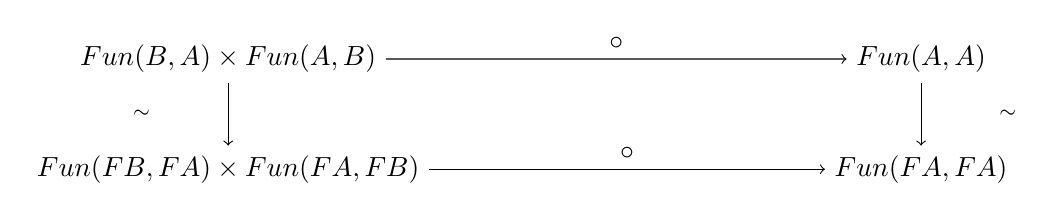
\begin{tikzpicture}[xscale=2.0,yscale=1.4]
\node (TL) at (0,1) {$\Fun(B,A)\times\Fun(A,B)$};
\node (TR) at (4.4,1) {$\Fun(A,A)$};
\node (BL) at (0,0) {$\Fun(FB,FA)\times\Fun(FA,FB)$};
\node (BR) at (4.4,0) {$\Fun(FA,FA)$};
\draw[->] (TL) -- (TR) node[midway,above]{$\circ$};
\draw[->] (TL) -- (BL);
\node at (-0.55,0.5) {$\scriptstyle\sim$};
\draw[->] (TR) -- (BR);
\node at (4.95,0.5) {$\scriptstyle\sim$};
\draw[->] (BL) -- (BR) node[midway,above]{$\circ$};
\end{tikzpicture}
\end{equation*}
在其\trHomotopyCategory{}之间诱导一个交换方块。特别地，
把复合双\trFunctor{}用于\trIsomorphism $Ff\cong\tilde{f}$ 与 $Fg\cong\tilde{g}$，
我们看到在 $\mathrm{h}(\Fun(A,A))$ 中
\[
F(\mathrm{id}_A)=\mathrm{id}_{FA}
\cong\tilde{g}\circ\tilde{f}
\cong Fg\circ Ff=F(g\circ f)
\]
由 $\mathrm{h}(\Fun(A,A))\rvEqArrow\mathrm{h}(\Fun(FA,FA))$
的全忠实性，这一\trIsomorphism\trLifting{}为 $\mathrm{h}(\Fun(A,A))$
中的\trIsomorphism $\mathrm{id}_A\cong g\circ f$。
由推论 1.1.16，%
这一\trIsomorphism{}可以由一个\trHomotopyCoherentIsomorphism $\mathbb{I}\to\Fun(A,A)$
表示，后者内部化而定义所需的映射
$\alpha\colon A\to A^{\mathbb{I}}$。
从 $f\circ g$ 到 $\mathrm{id}_B$ 的\trHomotopyCoherentIsomorphism
$\beta\colon B\to B^{\mathbb{I}}$ 之构造与此类似。
\end{proof}

\cref{lem:biequivalence-reflect-create} 中\trEquivalence{}之创造的证明出人意料地精细：
它转入\trFunctorSpace{}的\trHomotopyCategory{}，以避免\trLifting{}并复合\trHomotopyCoherentIsomorphism{}；
循此路线的论证也是可能的，
留作\cref{ex:biequivalence-creation-sketch}由读者完成。
下一节将通过引入\trInfinityCosmos{}的\trHomotopyTwoCategory{}%
为刚才给出的论证提供语境。随后请读者在练习 1.4.vi 中
重温\trEquivalence{}的创造。%

\subsection*{练习}

\begin{exercise}\label{ex:slice-induced-cosmological}
证明：对任何\trCosmologicalFunctor $F\colon\mathcal{K}\to\mathcal{L}$
与任何 $A\in\mathcal{K}$，
切片上诱导的映射 $F\colon\mathcal{K}_{/A}\to\mathcal{L}_{/FA}$
定义一个\trCosmologicalFunctor{}。
\end{exercise}

\begin{exercise}\label{ex:biequivalence-creation-sketch}
概述一个证明：宇宙论\trBiequivalence{}创造\trInfinityCategory{}之间的%
\trEquivalence{}而无须转入\trHomotopyCategory——办法是把作为所设%
\trEquivalence{}数据之一部分给出的那些\trHomotopyCoherentIsomorphism%
\trLifting{}并复合起来。
\end{exercise}

\begin{exercise}\label{ex:biequivalence-cancellation}
设 $F\colon\mathcal{K}\to\mathcal{L}$、
$G\colon\mathcal{L}\to\mathcal{M}$
与 $H\colon\mathcal{M}\to\mathcal{N}$
都是\trCosmologicalFunctor{}，并设 $GF$ 与 $HG$ 是宇宙论\trBiequivalence{}。
证明：$F$、$G$、$H$ 与 $HGF$ 都是宇宙论\trBiequivalence{}。
\end{exercise}
